%!TEX root = *.tex
%%%%%%%%%%%%%%%%%%
% メモ
\begin{comment}

\end{comment}
% カウンタのリセット
\setcounter{eqNo}{0}
\setcounter{figure}{0}
% 解答
\noindent {\large【解答】\par}
\noindent (1)\par 
\noindent\,(a)\,
導体内に一様な電場が生じており,その向きは高電位から低電位に向かう向きでA.
また,電場の大きさ$E$は$E=\dfrac{V}{L}$.

\noindent\,(b)\,
電子は電場から静電気力を受ける.
自由電子の電荷は負であり,電場とは反対の向きに力を受ける.
よって,静電気力の向きはBであり,力の大きさ$F$は,
\begin{align*}
  F = eE = \dfrac{eV}{L}
\end{align*}

\noindent (2)\par 
\noindent\,(c)\,
電子はBの向きに運動している.
電子の速さを$v_e$とすると,進行方向と反対の向きに大きさ$kv_e$の抵抗力を受けており,これが静電気力とつりあっている.
運動方程式
\begin{align*}
  0 = kv_e-\dfrac{eV}{L} \quad \therefore v_e = \dfrac{eV}{kL}
\end{align*}

{
\begin{wrapfigure}{r}{12zw}
  \vspace{-\intextsep}
  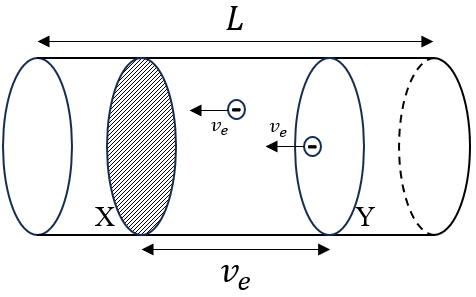
\includegraphics[width=12zw]{../graphs/jumon_111_sol.png}
  \caption{}
\end{wrapfigure}
\noindent\,(d)\,
導体内の断面Xを単位時間に通過する自由電子は,距離$v_e$だけ後方にある断面Yと断面Xの間に存在する.
XY間の体積は$Sv_e$なので,XY間に含まれる自由電子の数$N$は,
\begin{align*}
  N = n\times Sv_e = \dfrac{enSV}{kL}
\end{align*}

\par}

\noindent\,(e)\,
電流の大きさ$I$は,断面Xを単位時間あたりに通過する電気量ゆえ,
\begin{align*}
  I = eN = \dfrac{e^2nSV}{kL}
\end{align*}

\noindent\,(f)\,
(e)の結果から,導体の抵抗$R$は
\begin{align*}
  R = \dfrac{V}{I} = \dfrac{kL}{e^2nS}
\end{align*}

\noindent (3)\par 
\noindent\,(g)\,
電場が1個の自由電子に対して単位時間に行う仕事$P_e$は,
自由電子が静電気力から受ける仕事率であり,
\begin{align*}
  P_e = Fv_e = \dfrac{e^2V^2}{kL^2}
\end{align*}

\noindent\,(h)\,
導体中のすべての自由電子($nSL$個)が電場からうける仕事率$P$が導体から単位時間に発生するジュール熱である.
\begin{align*}
  P = nSL\cdot P_e = \dfrac{e^2nSV^2}{kL}
\end{align*}

%%%%%%%%%%%%%%%%%%